\documentclass[11pt]{article}
\usepackage{my_syllabus}


 \author{Joshua Bowles}
\title{Research Links\\
\small Eng 2020; Spring 2010}
\date{\today}

\begin{document}
\maketitle

%\includegraphics[width=1in]{madscientistmuppet}\includegraphics[width=2in]{UVU_Horizontal_Mark_1-color}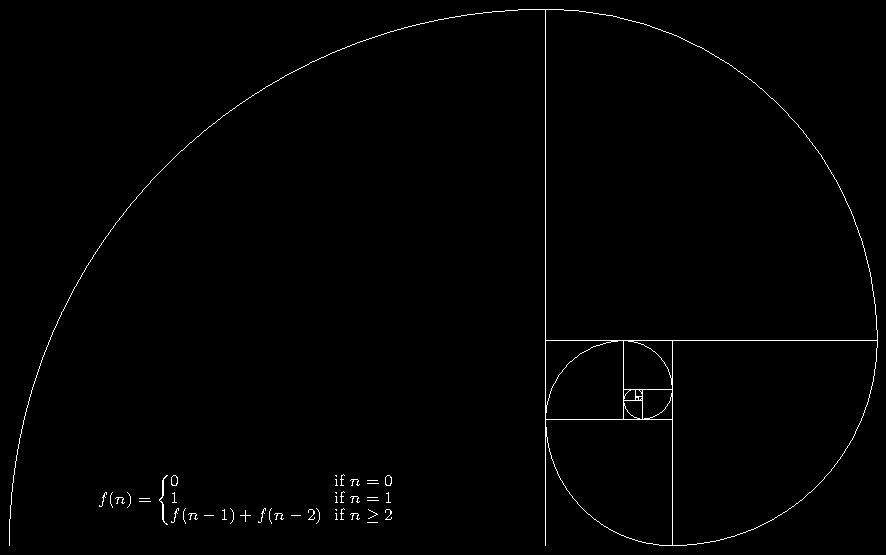
\includegraphics[width=2in]{fibonacci-spiral}\includegraphics[width=1in]{Rplot001}

  \section{Basic Resources}
The following is a list (with active links) of some basic research corpora.
  \begin{itemize}
\item UVU library: \href{http://www.uvu.edu/library}{http://www.uvu.edu/library}
\item Library search engines: \href{http://www.uvu.edu/library/search/index.php}
{http://www.uvu.edu/library/search/index.php}
\item Useful databases: JSTOR, MEDLINE, especially ACADEMIC SEARCH PREMIER
\item Cornell science archive: \href{http://www.arXiv.org}{http://www.arXiv.org}
\item UVU writing center: \href{http://www.uvsc.edu/owl}{http://www.uvsc.edu/owl}
\end{itemize}

\section{Databases}\begin{itemize}  
\item Research tools accessible at the \href{http://www.uvu.edu/library/researchtools/index.html}{UVU-Library}
\item \href{http://www.uvu.edu/library/guides/index.html}{Research guides} by topic at UVU library
\item \href{http://www.uvu.edu/library/researchtools/electronic_encyclopedias.html}{Electronic Encyclopedias and 
Dictionaries}
\item JSTOR 
\item ScienceDirect 
\item ERIC 
\item Academic Search Premier 
\item Project Muse
\end{itemize}

\subsection{Other Links and Sources}
\begin{itemize}
\item \href{http://languagelog.ldc.upenn.edu/nll/}{Language Log}
\item \href{http://mitpress.mit.edu}{MIT Press} 
\item \href{http://arxiv.org}{Cornell ArXiv} 
\item \href{http://plato.stanford.edu/}{Stanford Encyclopedia of Philosophy} 
\item Academic web pages of \href{http://www.uvu.edu/profpages/profiles/show/user_id/530}{professors} 
for downloadable papers\footnote{Make sure these sites are connected to a University or College---as 
the example here shows, if you are on-line!}
\end{itemize}

\end{document}